\documentclass[12pt,a4paper]{report}
\usepackage[T2A]{fontenc}
\usepackage[utf8]{inputenc}
\usepackage[russian]{babel}
\usepackage{graphicx, setspace, amsmath, amsfonts}

\usepackage[
top = 1.25cm, 
bottom = 2.0cm]{geometry}

\begin{document}
\begin{titlepage} 
	\centering
    % HEADER
	{
        \scshape
        Федеральное государственное автономное образовательное учреждение высшего образования
        \par
        \textbf{«Научно-образовательная корпорация ИТМО»}
        \par
        \vspace*{1cm}
        Факультет Программной Инженерии и Компьютерной Техники
        \par
    }
    % LOGO
    \vspace*{0.6cm}
    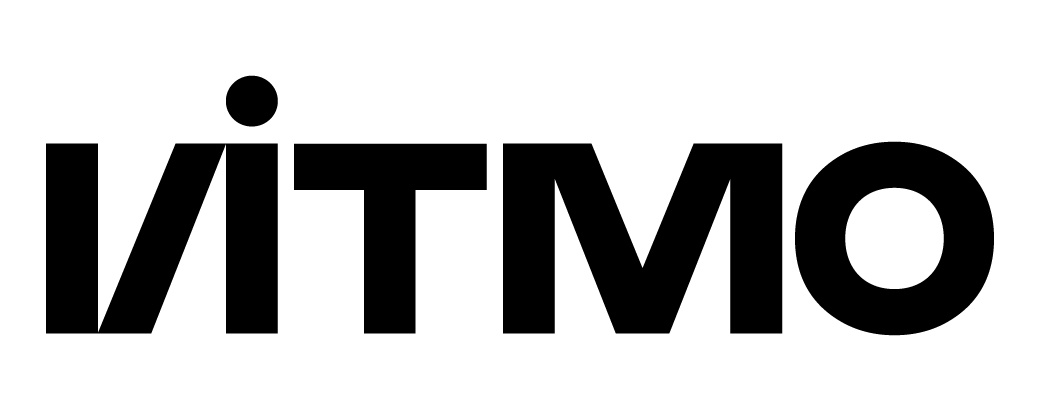
\includegraphics[width=\textwidth]{logo.png}
    % LAB INFO
    {
        \Large
        \textbf{Курсовая работа по нечёткой логике}
        \par
        \normalsize
        \vspace*{0.75cm}
        \textbf{}
        \par
    }
    \vfill
    % СREDITS
    \hfill\begin{minipage}{\dimexpr\textwidth-7.8cm}
        \textbf{Выполнил:}\par
        Степанов Арсений Алексеевич\par
        \vspace*{0.15cm}
        \textbf{Группа:}\par
        P3109\par
        \vspace*{0.15cm}
        \textbf{Преподаватель:}\par
        Поляков Владимир Иванович\par
    \end{minipage}
    \vfill
    Санкт-Петербург, \the\year{}г.
\end{titlepage}   
\onehalfspacing
\section*{Постановка задачи}
Разработать алгоритм, по которому определяется рекомендуемый тип обуви для покупки, исходя из текущей погоды и текущего бюджета
\subsection*{Входные данные}
\begin{itemize}
    \item Погода
    \item Бюджет
\end{itemize}
\subsection*{Выходные данные}
\begin{itemize}
    \item Тип обуви
\end{itemize}
\newpage
\section*{Фазификация}
\subsection*{Входные данные}
\subsubsection*{Погода}
Погода определяется текущей температурой на улице, для неё введём следующие обозначения:
\begin{itemize}
    \item CD (cold) - холодная погода (соответствует зиме)
    \item MD (mild) - умеренная погода (соответствует весне/осени)
    \item HT (hot)  - жаркая погода (соответствует лету)
\end{itemize}
\subsubsection*{Бюджет}
Бюджет определяется количеством денег, которые предполагаются быть потраченными на покупку обуви, для этого введём следующие обозначения:
\begin{itemize}
    \item LT (little) - небольшое количество денег
    \item MT (moderate) - среднее количество денег
    \item MN (many)  - большое количество денег
\end{itemize}
\subsection*{Выходные данные}
Рекомендуемый к покупке тип обуви рассчитанный на основе текущего бюджета и погоды
\begin{itemize}
    \item FT (felt boots) - валенки
    \item BT (boots) - боты
    \item LB (leather boots) - кожаные ботинки
    \item BS (bast shoes) - лапти
    \item SK (sneakers) - кроссовки
    \item SP (slippers) - шлёпанцы
    \item SD (sandals) - сандали
\end{itemize}
\newpage
\section*{Выработка решения}
\subsection*{Функция принадлежности для погоды}
\begin{center}
\includegraphics*[height=5cm]{func_1.jpg}    
\end{center}
$M_{CD}(X) = -x+1$, $x \in [0, 1]$ \\
$M_{MD}(X) = - |x-1.5|+1$, $x \in [0.5, 2.5]$ \\
$M_{HT}(X) = x-2$, $x \in [2, 3]$ \\
\subsection*{Функция принадлежности для бюджета}
\begin{center}
\includegraphics*[height=5cm]{func_2.jpg}    
\end{center}
$M_{LT}(y) = -y+1$, $y \in [0, 1]$ \\
$M_{MT}(y) = - |y-1.5|+1$, $y \in [0.5, 2.5]$ \\
$M_{MN }(y) = y-2$, $y \in [2, 3]$ \\
\newpage
\subsection*{Функция принадлежности для типа обуви}
\begin{center}
\includegraphics*[width=15cm]{func_3.jpg}    
\end{center}
$M_{FT}(z) = -z+1$, $z \in [0, 1]$ \\
$M_{BT}(z) = - |z-1.5|+1$, $z \in [0.5, 2.5]$ \\
$M_{LB}(z) = - |z-3|+1$, $z \in [2, 4]$ \\
$M_{BS}(z) = - |z-4.5|+1$, $z \in [3.5, 5.5]$ \\
$M_{SK}(z) = - |z-6|+1$, $z \in [5, 6]$ \\
$M_{SP}(z) = - |z-7.5|+1$, $z \in [6.5, 8.5]$ \\
$M_{SD}(z) = z-8$, $z \in [8, 9]$ \\
\subsection*{База правил}
Зададим базу правил для условий:\\
\hfill\break
\begin{tabular}{|c||c|c|c|}
    \hline
       & CD & MD & HT \\
    \hline
    \hline
    LT & FT & BS & SP \\
    \hline
    MT & BT & SK & SD \\
    \hline
    MN & LB & SK & SD \\
    \hline
\end{tabular}
\subsection*{Оценка правил}
Допустим Валерию Альбертовичу надо определиться с покупкой обуви в конце мая 
с довольно ограниченным бюджетом\\
Погоду в мае можно оценить в 2.1, а бюджет как 0.6\\
Тогда нужно оценить следующие правила:
\begin{itemize}
    \item Умеренная погода и небольшой бюджет
    \item Умеренная погода и средний бюджет
    \item Жаркая погода и небольшой бюджет
    \item Жаркая погода и средний бюджет
\end{itemize}
Определим степень истинности каждого условия:
\begin{itemize}
    \item $S_1=\min(M_{MD}(2.1), M_{LT}(0.6))=\min(0.4, 0.4)=0.4$
    \item $S_1=\min(M_{MD}(2.1), M_{MT}(0.6))=\min(0.4, 0.1)=0.1$
    \item $S_1=\min(M_{HT}(2.1), M_{LT}(0.6))=\min(0.1, 0.4)=0.1$
    \item $S_1=\min(M_{HT}(2.1), M_{MT}(0.6))=\min(0.1, 0.1)=0.1$
\end{itemize}
Таким образом получаем что наибольшая степень истинности соответствует паре MD и LT, что соответствует значению BS
\section*{Дефазификация}
Вычислим итоговое значение: \\
\hfill\break
$M(z)=- |z-4.5|+1$ \\
$0.4=- |z-4.5|+1$, $z_1=3.9$, $z_2=5.1$ \\
$z_{avg}=4.5$ \\
\hfill\break
Таким образом получаем что если Валерию Альбертовичу в текущей жизненной ситуации понадобится купить обувь, то ему стоит подумать над приобретением пары лаптей
\end{document}
